\section{Using BoAT-v2}
\label{sec:annotation}

\begin{figure}[th!]
    \centering
    \tcbox[left=0mm,right=0mm,top=0mm,bottom=0mm,boxsep=1pt,arc=0mm,boxrule=0.5pt,colframe=black,sharp corners]
    {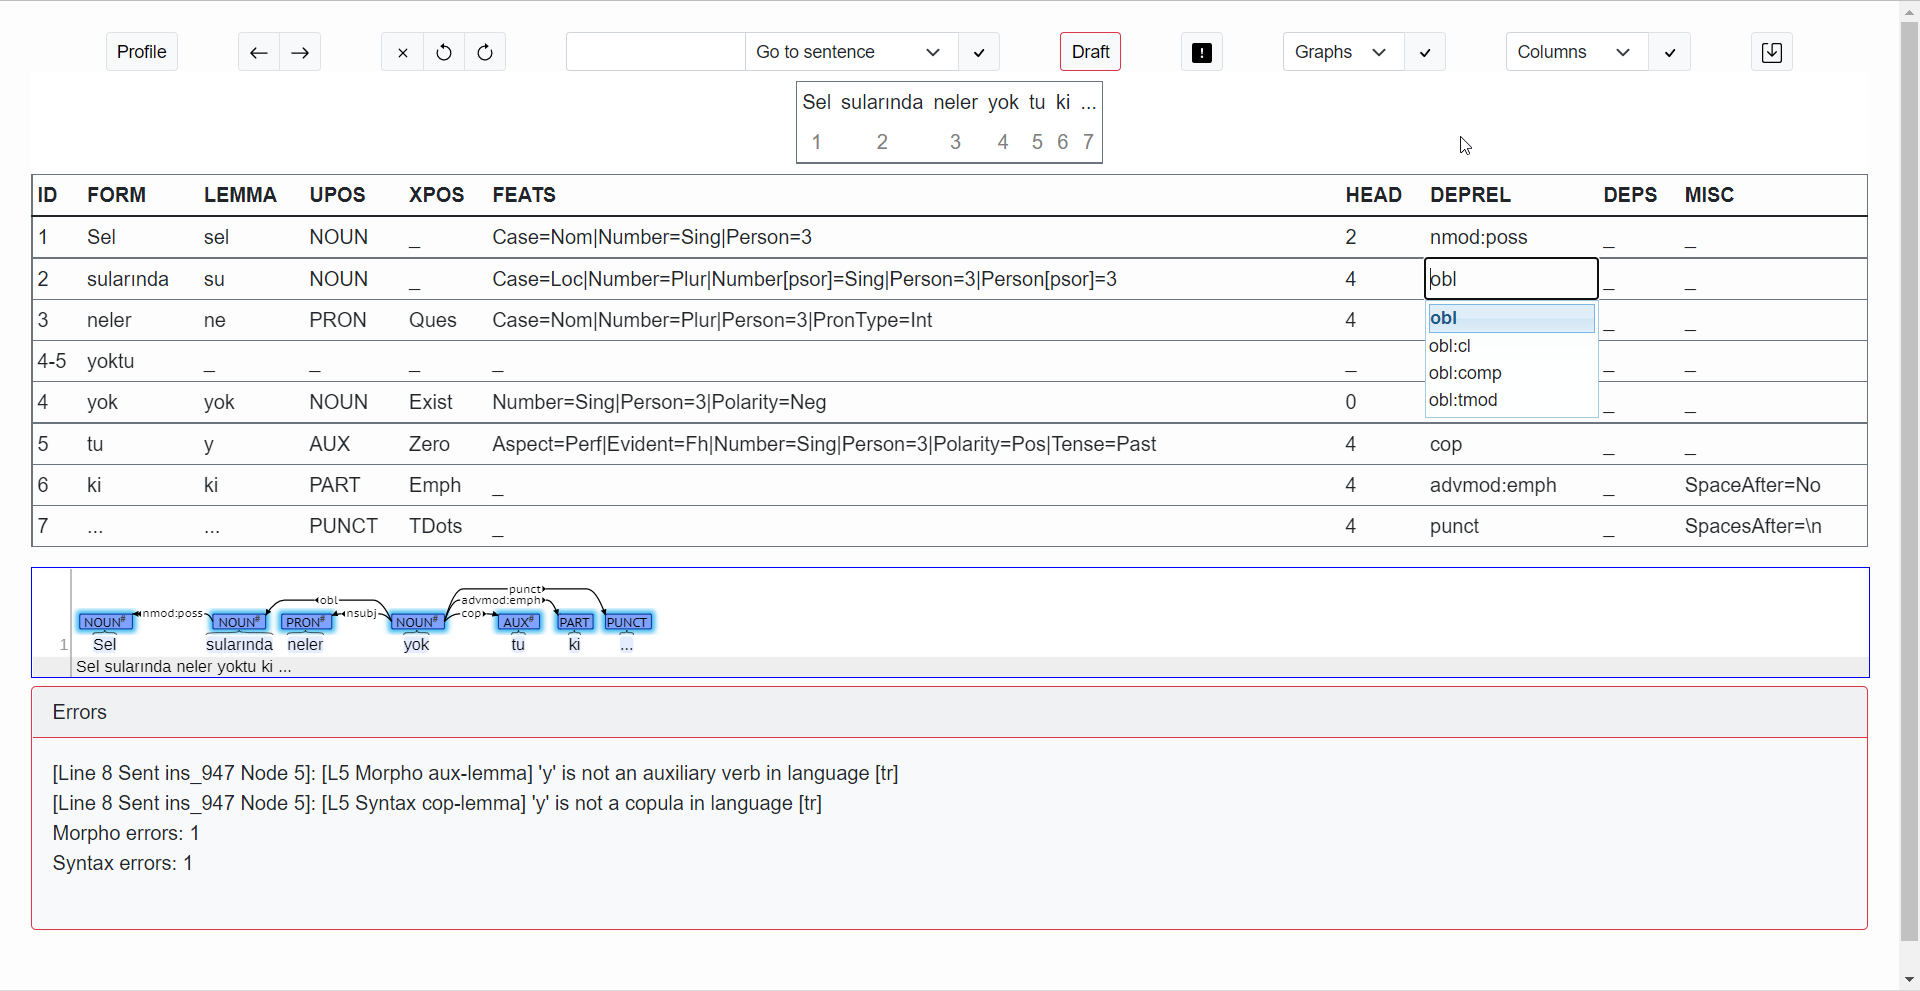
\includegraphics[width=1\textwidth]{figures/boat-v2-sample-annotation.png}}
    \caption{The annotation screen captured while the sentence ``Sel sularında neler yoktu ki...'' is being annotated. The \deprel\ tag for the surface form ``sularında'' is being annotated by selecting among the valid alternatives that appear in the pop-up. Selections can be made with the use of arrow keys.}
    \label{fig:anno-fig}
\end{figure}

A typical annotation can proceed as follows:
An annotator selects a sentence from a treebank.
An annotation table appears with the sentence parsed according to the \ud\ format.
Each row corresponds to a token and its annotations.
Figure~\ref{fig:anno-fig} shows the annotation view while an annotator is annotating a Turkish sentence ``Sel sularında neler yoktu ki...'' (translation: \textit{What wasn't in the flood waters...}).

An annotator can make use of dependency graphs, errors, and search during annotation.
Dependency graphs are visual cues for how lemmas are dependent upon one another.
Errors are helpful reminders compliant with \ud.

Annotators can customize the columns and dependency graph in accordance with their preferences.
When an annotation is finished, its status can be set to ``Complete''.
The annotator can search for previously made annotations in combinations of text and feature values to refer to previously made annotations.
